\chapter{Algorithm Design} \label{chap:Algorithm Design}

\section{Algorithm Overview}
The primary focus of this research is to develop an accurate KNN
Join algorithm for spark framework. The decision to use spark as our
framework is driven by
the fact that spark is in memory and runs much faster than Hadoop
Mapreduce. The same sentiment is also being echoed in the industry as
well, as we see more companies are moving to spark from Hadoop map
reduce.

We have few basic assumptions about the dataset R and S.
\begin{enumerate}
\item Both S and R dataset is large
\item S dataset is stable but R can be changing
\item S dataset is larger than R dataset
\item Number of dimensions is less (in order of 10s)
\end{enumerate}


\begin{figure}[t!]
  \caption{Voronoi Partition}
  \label{voronoi_partition}
  \centering
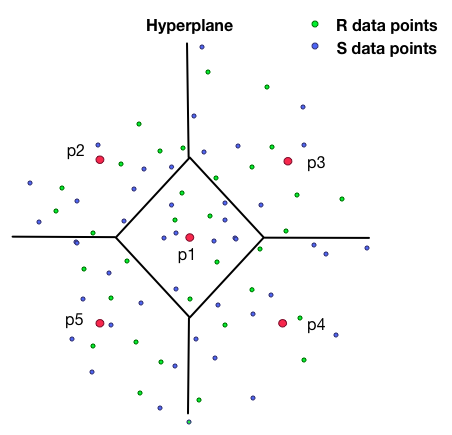
\includegraphics[width=10cm,height=10cm]{images/voronoi.png}
\end{figure}


\begin{center}
\begin{figure}
\begin{tikzpicture}
\draw[blue] (0,0) circle (4pt) ;
\draw[blue] (4,0) circle (4pt);
\draw[black]  (3, 1.5) circle (4pt);
\draw[red]   (3.65, 2.2) circle (4pt);

\draw[thin] (3,1.5)node[right]{$\mathbf{r_i}$} -- (0, 0) node[left]{$\mathbf{O_j}$} -- (4,0) node[right]{$\mathbf{O_i}$};
\draw[thin] (4, 0) -- (3, 1.5);
\draw[thin] (3, 1.5) -- node[above]{$\mathbf{y}$} (3.65, 2.2) ;
\draw[thin,dashed] (3, 1.5) -- node[above]{$\mathbf{x}$} (2, 1.5) ;
\draw[thick] (2,3) -- (2,-1) node[right]{$\mathbf{HP(O_i, O_j)}$} ;

\node[text width=6.2in] at (2,-2) {$x = \frac{|p,\ O_i|^2\ -\ |p,\ O_j|^2}{2 \times |O_i,\ O_j|}$};
\node[text width=6.2in] at (2,-3) {y = distance of farthest neighbour};
\end{tikzpicture}
\caption{ Distance bound for a point to its hyperplane }
\label{fig_triangle_inequality}
\end{figure}
\end{center}


In spark to run the algorithm in parallel, we need to split the data
into partitions. This way each partition can be loaded into separate
nodes and processed in parallel. Partitioning the dataset helps us to run
the algorithm even if the dataset cannot fit into the RAM of single
node. Spark provides a way to partition the data as we deemed necessary.
In our algorithm we partition the data by first selecting a set of
random pivots. All the vectors which are near to a pivot forms a
partition. Such partition is called voronoi partition [Figure ~\ref{voronoi_partition}]. Both R and S
dataset is partitioned using the same pivots.

The central
idea for our algorithm is if a vector is at the center of the partition
then most likely the neighbours are within the same partition. This
computation is done using join transformation in spark. We join
the R and S dataset, and find the nearest neighbours for partition
$R_i$ in $S_i$. For smaller dimension data nearly 50 to 60 percentage
of the vector in R finds its k nearest neighbours in the same
partition in S dataset. Once we find the nearest neighbour for every
vector we check if the distance to farthest neighbour is greater than
the distance to border separating two partitions. If the distance is
greater then we consider that the vector is at the edge of the
partition else the vector is at center of the partition [Figure ~\ref{fig_triangle_inequality}].

For the vectors which are near to the edge of the partition, we
iteratively look for nearest neighbours in nearby partitions and
update the previously computed results. This way the algorithm can
stop once we have checked all the nearest partition or found the best
K nearest neighbours.

Since we are partitioning the data into n partitions, horizontal scalability we can
be as high as n nodes. This is the level of parallelism that
the algorithm provides. Empirically limiting the size of the
partition to be between 1000 to 3000 elements, provides best run time.

\section{Detailed Steps}

In this section we will provide a detailed description of our
algorithm.

The algorithm has two phases
\begin{enumerate}
\item Pivot Selection and Partition
\item Join
\end{enumerate}

\subsection{Pivot Selection and Partition}
The first step of our algorithm is to partition the R and S data into smaller
subsets. This is a data preprocessing step. This step is crucial for
two reasons

\begin{enumerate}
\item Better Partition gives better run time performance
\item Partition also helps us in horizontal scalability
\end{enumerate}

Pivot selection has been studied in depth in \cite{lu_efficient_2012}.
In that paper, three different strategies were employed and
evaluated. The strategies are
\begin{enumerate}
\item Random Selection
\item Farthest Selection
\item K Means Selection
\end{enumerate}

Out of these three, K Means provides the best standard deviation of
partition size. Random selection provided the next best results. But
computation time needed for K Means is higher than Random
Selection. Based on those results from \cite{lu_efficient_2012}, we
chose to employ Random Selection for our pivot selection.

There is minor deviation in which dataset to be used for selecting
pivots. \cite{lu_efficient_2012} uses R dataset for pivot
selection. But we chose to use S dataset for pivot selection. This is
because practically S dataset remains stable and R dataset changes. So
if we chose pivots selection on S dataset we can reuse the
results. This will speed up time when we do KNN Join of multiple R
dataset with S.

\medskip

Below is the pseudocode for Random Pivot selection algorithm.

\begin{algorithm}
  \caption{Random Pivot Selection}
  \label{algo_pivot_selection}
  \algsetup{linenosize=\small}
  \begin{algorithmic}[1]
    \FOR{$i=0$ to $i=T$}
    \STATE $P_i  \leftarrow \ N\ Random\ Points\ v^i_1,v^i_2,...v^i_N  from\ S$
    \STATE $T_{dist}^i \leftarrow \sum\limits_{x=0}^N\sum\limits_{y=x}^N d(v^i_x, T^i_y)$
    \ENDFOR
    \STATE $pivots \leftarrow\ T^i$ where $T^i\ has\ max\ T^i_{dist}$
  \end{algorithmic}
\end{algorithm}


In Random Pivot selection algorithm [~\ref{algo_pivot_selection}], we randomly pick N Pivots from the
S dataset. We pick T such random sets {$P_1$,$P_2$, ... $P_T$}. For each set $P_i$, We
compute the distance between every two
vectors and take a cumulative sum. Finally We select the set $P_i$
which has the maximum cumulative sum.

\bigskip

After selecting the pivots, next step is to partition the S dataset
and R dataset. Below is the pseudocode for data partitioning.

\begin{algorithm}
  \caption{Dataset Partition}
  \label{algo_dataset_partition}
  \algsetup{linenosize=\small}
  \begin{algorithmic}[1]
    \STATE $DS\ \leftarrow\ input\ dataset$
    \FORALL{$v\ in\ DS$}
    \STATE v.partitionId = $min_{O_i \forall O}\{dist(v, O_i)\}$.pivotIndex
    \ENDFOR
  \end{algorithmic}
\end{algorithm}


For every point in the dataset we find the nearest pivot. All
the points that is closer to the pivot forms a partition. We also
cache the partitioned dataset. This is to avoid recomputation in
spark.

In spark we create a RDD for both S and R Dataset. The RDD is
partitioned based on our data partition algorithm
[~\ref{algo_dataset_partition}]. The RDD has N elements, each element is
made as a partition. The element is of
the format \emph{(partitionId, List(vectors))}. This format helps us
while we do join between R and S dataset. We use hash partitioner to
make sure elements with same key are colocated. Hence the partition $r_i$ and
$s_i$ will be colocated since they have the same partitionId.

\medskip

\begin{algorithm}
  \caption{Summary Table}
  \label{algo_generate_summary}
  \algsetup{linenosize=\small}
  \begin{algorithmic}[1]
    \FORALL{$S_i\ in\ S$}
    \STATE $S_i$.maxDistance = $max_{s_i \forall S_i}\{dist(s_i, O_i)\}$
    \ENDFOR
  \end{algorithmic}
\end{algorithm}

Once we have partitioned R and S dataset, we create a summary
table. In summary table we find the max distance of a vector from a
pivot. This information is later used while calculating whether the
vector is at the center or at the edge.

\subsection{Join}

\medskip

Theorem1: \cite{lu_efficient_2012} \\

Given two pivots $O_i$, $O_j$ of two voronoi
partition $S_i$ and $S_j$, Let HP($O_i$, $O_j$) be a generalized
hyperplane which is equidistant from $O_i$ and $O_j$. Then $\forall\ p\
\epsilon\ R_j$

\medskip

\begin{center}

$d(p, HP(O_i, O_j))$ = $\frac{|p, O_i|^2 - |p, O_j|^2}{2 \times |O_i, O_j|}$

\end{center}

\bigskip

Corollary1: \\

Given a point $p\ \epsilon\ R_j$, $\theta = \max{d(p, KNN(p, S_j))}$ be max K Nearest
neighbour distance from p in partition $S_j$ then partition
$R_i$ can contain nearest neighbour only if

\medskip

\begin{center}

$d(p, HP(O_i, O_j)) > \theta $

\end{center}


\begin{algorithm}
  \caption{Bruteforce NN}
  \label{algo_bruteforce_nn}
  \algsetup{linenosize=\small}
  \begin{algorithmic}[1]
    \STATE $S_i \leftarrow input$
    \STATE $R_i \leftarrow input$
    \FORALL{$r_x\ in\ R_i$}
    \STATE $r_x$.KNN = []
    \FORALL{$s_y\ in\ S_j$}
    \STATE dist = |$r_x$, $s_y$|
    \IF {dist < |$r_x$, $r_x$.KNN[last]|}
    \STATE $r_x$.KNN[last] = $s_y$
    \ENDIF
    \ENDFOR
    \ENDFOR
  \end{algorithmic}
\end{algorithm}


In this phase we start with a join transformation between R
and S dataset. Spark's Join Transformation when called on two dataset R and S,
which is of format (K, V) and (K, W) respectively returns (K,
(V,W)). Since we have R and S dataset partitioned into N partitions,
with the format of each element being (partitionId, List($r_i$)) and
(partitionId, List($s_i$)), join transformation produces (partitionId,
(List($r_i$), List($s_i$))). Since the data is colocated there will not
be any shuffle due to join transformation. We perform bruteforce KNN
Join on the joined output. So we find K Nearest neighbour for all
elements in $R_i$ within $S_i$. Since the size of $S_i$ and $R_i$ are
small, the bruteforce gives faster results. The pseudocode for
BruteForce KNN is shown in Algorithm ~\ref{algo_bruteforce_nn}.

\begin{algorithm}
  \caption{FindNbrPartition}
  \label{algo_nbr_partition}
  \algsetup{linenosize=\small}
  \begin{algorithmic}[1]
    \FORALL{$R_i\ in\ R$}
    \FORALL{$r_x in R_i$}
    \STATE $r_x$.nbrPart = []
    \FORALL{$O_j in O$ }
    \STATE $x = \frac{|r_x,\ O_i|^2\ -\ |,\ O_j|^2}{2 \times |O_i,\
      O_j|}$
    \IF{x < $r_x$.KNN[last]}
    \STATE $r_x$.nbrPart.append($R_i$)
    \ELSE
    \STATE $r_x$ has all its KNN Found
    \ENDIF
    \ENDFOR
    \ENDFOR
    \ENDFOR
  \end{algorithmic}
\end{algorithm}



Now having computed the K Nearest neighbour within the partition, next
step is to find for every vector in $R_i$, the nearest
partitions which may contain Nearest Neighbours. From ~\ref{fig_triangle_inequality}, we can see that if $x > y
$ then the partition will not contain any neighbours for the vector
$r_i$. If $x < y$ then the partition might contain a neighbour, so we
select the partition for further inspection. The pseudocode for
Finding then neighbour partition is given by Algorithm ~\ref{algo_nbr_partition}

\begin{algorithm}
  \caption{Partition and Join}
  \label{algo_join}
  \algsetup{linenosize=\small}
  \begin{algorithmic}[1]
    \REPEAT

    \FORALL{i=0 to N}
    \STATE Call BruteforceNN($R_i$,$S_i$)
    \ENDFOR

    \STATE Call FindNbrPartition

    \FORALL{r in R}
    \STATE Move r to r.nbrPart[0]
    \ENDFOR

    \UNTIL{KNN Found for all $r \in R$}

  \end{algorithmic}
\end{algorithm}


\bigskip

The pseudocode for the join phase is given by Algorithm ~\ref{algo_join}.
For every partition $R_i$,
$S_j$ where $i=j$ we find K nearest neighbours for all points in
$R_i$ within $S_i$. We also find other partitions for $R_i$ in $S_j$
$\forall\ i\ \neq\ j$ where there is a possibility of finding
neighbours. For this we use the Theorem1 and Corollary1.
Once we find the nearest partition we move the $r \in R$ to that partition
and search for the nearest neighbour in that.

In Each iteration in the loop starting at line number 6, more and more elements in R will have its nearest
neighbour found. If the amount of elements in R is small, it will be
faster if we replicate the element in R to all the nearest\_partition
and finding nearest neighbours in each partition and finally combining
it. This proved to provide significant improvement in performance.

\bigskip

%%% Local Variables:
%%% mode: latex
%%% TeX-master: t
%%% End:
